\documentclass[11pt,a4paper]{article}
\usepackage[margin=1in]{geometry}
\usepackage[T1]{fontenc}
\usepackage[utf8]{inputenc}
\usepackage{lmodern}
\usepackage{hyperref}
\usepackage{enumitem}
\usepackage{xurl}
\usepackage{tikz}
\usepackage{float}
\usetikzlibrary{arrows.meta, positioning, shapes.geometric}
\hypersetup{colorlinks=true,linkcolor=blue,urlcolor=blue}
\newcommand{\codepath}[1]{\path{#1}}
\tikzset{
  box/.style={rectangle,draw,rounded corners,align=center,inner sep=3pt,minimum width=44mm},
  decision/.style={diamond,draw,aspect=2.2,align=center,inner sep=2pt},
  line/.style={-Latex}
}

\title{Phase-2 QEMU: Deliverable 4 (Golden Micro-kernel Traces)}
\author{SIT Engine Documentation}
\date{\today}

\begin{document}
\maketitle

\section{Technical Description}
QEMU golden traces provide deterministic replay anchors to detect parser/engine regressions independently from workload churn.

\section{Implementation Fulfillment}
Trace generation uses pipeline entry \texttt{run\_qemu\_golden\_pipeline.main()} and per-case execution through \texttt{riscvbench.main()}; replay validation is performed by \texttt{run\_golden\_suite.main()}.

\section{Design \& Architecture}
\subsection*{Function Attributes}
\begin{itemize}[leftmargin=*]
  \item \texttt{run\_qemu\_golden\_pipeline.main()}: Inputs=workload/size/flag matrix; Outputs=QEMU trace bundle + index; Side effects=orchestrates target golden cases; Failure modes=matrix run failures.
  \item \texttt{riscvbench.main()}: Inputs=single case config; Outputs=normalized trace + run artifacts; Side effects=executes target case; Failure modes=toolchain/runtime failure.
  \item \texttt{build\_manifest()}: Inputs=trace paths + masks + window; Outputs=manifest JSON; Side effects=pins replay inputs; Failure modes=missing paths/metadata.
  \item \texttt{run\_golden\_suite.main()}: Inputs=manifest/outdir; Outputs=replay pass/fail; Side effects=confirms replayability; Failure modes=replay/invariant errors.
\end{itemize}
\subsection*{Function Execution Details}
\begin{enumerate}[leftmargin=*]
  \item \texttt{run\_qemu\_golden\_pipeline.main()}
  \begin{itemize}[leftmargin=*]
    \item Input attributes: workload/size/flag matrix.
    \item Processing flow: orchestrates target golden cases.
    \item Output attributes: QEMU trace bundle + index.
    \item Failure behavior: matrix run failures.
  \end{itemize}
  \item \texttt{riscvbench.main()}
  \begin{itemize}[leftmargin=*]
    \item Input attributes: single case config.
    \item Processing flow: executes target case.
    \item Output attributes: normalized trace + run artifacts.
    \item Failure behavior: toolchain/runtime failure.
  \end{itemize}
  \item \texttt{build\_manifest()}
  \begin{itemize}[leftmargin=*]
    \item Input attributes: trace paths + masks + window.
    \item Processing flow: pins replay inputs.
    \item Output attributes: manifest JSON.
    \item Failure behavior: missing paths/metadata.
  \end{itemize}
  \item \texttt{run\_golden\_suite.main()}
  \begin{itemize}[leftmargin=*]
    \item Input attributes: manifest/outdir.
    \item Processing flow: confirms replayability.
    \item Output attributes: replay pass/fail.
    \item Failure behavior: replay/invariant errors.
  \end{itemize}
\end{enumerate}


\subsection*{Diagram A: End-to-End Design Flow}
\begin{figure}[H]
\centering
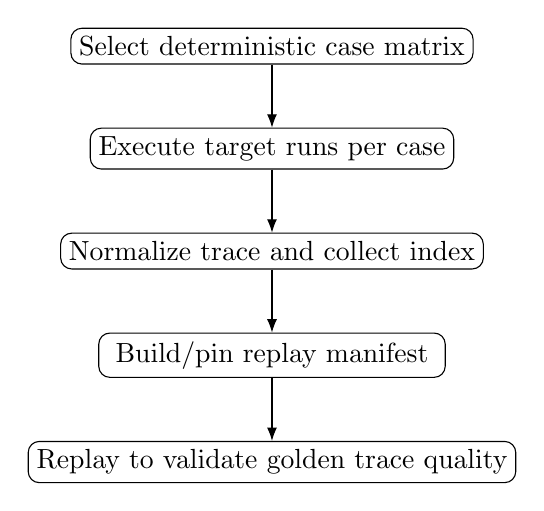
\begin{tikzpicture}[node distance=8mm and 12mm]
\node[box] (a) {Select deterministic case matrix};
\node[box, below=of a] (b) {Execute target runs per case};
\node[box, below=of b] (c) {Normalize trace and collect index};
\node[box, below=of c] (d) {Build/pin replay manifest};
\node[box, below=of d] (e) {Replay to validate golden trace quality};
\draw[line] (a) -- (b);
\draw[line] (b) -- (c);
\draw[line] (c) -- (d);
\draw[line] (d) -- (e);
\end{tikzpicture}
\caption{QEMU Deliverable 04: End-to-End Design Flow}
\end{figure}

\subsection*{Diagram B: Function Interaction and Attribute Flow}
\begin{figure}[H]
\centering
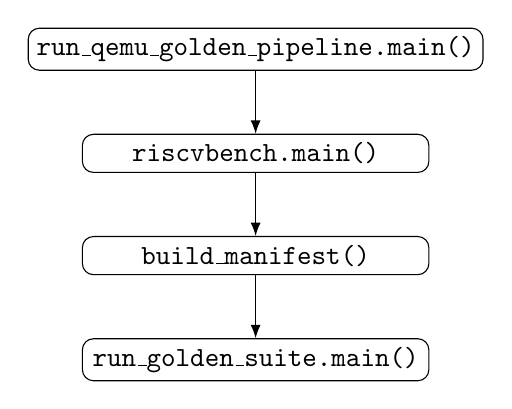
\begin{tikzpicture}[node distance=8mm and 12mm]
\node[box] (fa) {\texttt{run\_qemu\_golden\_pipeline.main()}};
\node[box, below=of fa] (fb) {\texttt{riscvbench.main()}};
\node[box, below=of fb] (fc) {\texttt{build\_manifest()}};
\node[box, below=of fc] (fd) {\texttt{run\_golden\_suite.main()}};
\draw[line] (fa) -- (fb);
\draw[line] (fb) -- (fc);
\draw[line] (fc) -- (fd);
\end{tikzpicture}
\caption{QEMU Deliverable 04: Function Interaction and Attribute Flow}
\end{figure}

\end{document}
